\section{Présentation}
Un algorithme intuitif pour résoudre un problème SAT serait de calculer la
table de vérité de la formule booléenne. On aurait donc une complexité
exponentielle. Si c'est acceptable sur des nombres très restreints de
variables, cela devient inacceptable dès que les problèmes commencent à
grandir. \todo{Indiquer le nombre de variables dans la résolution du HIPP}

Au vu du nombres d'utilisations de ce problèmes, un algorithme plus efficace
est recherché. Cependant, le problème étant $NP$-complet, il est fort probable
qu'une solution en temps polynomial dans le pire des cas n'existe pas.

Afin de compenser cette limite, de nombreuses techniques ont été développée
pour avoir des performances acceptables \todo{Une quantification des
performances actuelles} sur des problème ayant des dizaines de milliers de
variables et des millions de clauses.
\idee{Étudier les solveurs non complets}

Nous allons donc maintenant présenter un certain nombre des méthodes utilisées.
\idee{Adapter les algorithmes pour une résolution accélérée du problème HIPP}

\section{Techniques}
\subsection{Simplifications}
Afin de diminuer le nombre de clauses et le nombre de tests nécessaires,
certaines simplifications peuvent être faite sur les clauses, en utilisant les
règles suivantes : \begin{itemize}
    \item Résolution :
           $(x_1\vee\alpha) \wedge (\neg x_1\vee\beta) \equiv \alpha\vee\beta$
    \item $x \vee x \equiv x$
    \item $(\alpha\vee\beta)\wedge\alpha\equiv\alpha$
    \item $x\vee\neg x \equiv \bot$
\end{itemize}
\demo{Équivalence ou cosatisfiabilité ?}

Le premier algorithme utilisait uniquement la méthode de résolution : c'était
l'algorithme de \emph{Davis-Putnam}\cite{dp60}. Cet algorithme
consistait en la sélection d'une variable, à appliquer la résolution sur toute
les paires de la forme $x\vee\alpha$ et $\neg x\vee\beta$, puis à supposer
$x$ soit vrai soit faux (ce qui revient à supprimer les clauses contenant $x$
ou celles contenant $\neg x$), puis à itérer jusqu'à obtenir la clause vide
(valant $\bot$), ou la formule vide (valant $\top$). Si l'une des branches de
calcul permet d'obtenir la formule vide, la formule est \texttt{SAT}, dans le
cas contraire elle est \texttt{UNSAT}.

Une autre simplification possible est celle de la \emph{variable pure}. Une
variable est dite \emph{pure} si elle n'apparait que directement ou niée, mais
jamais les deux. Auquel cas elle peut être supposée toujours vraie ou fausse,
et permet de supprimer les clauses où elle intervient. Cette simplification
ne préserve pas l'équivalence logique mais la satisfiabilité.

\subsection{Backtracking}\label{back}
Afin de réduire les coûts en mémoire, les algorithmes peuvent se faire de
façon récursive, en choisissant une variable, faisant les simplifications qui
s'imposent et en remontant d'un cran si le résultat est \texttt{UNSAT}. Cette
méthode a été introduite par \emph{Davis}, \emph{Logemann} et \emph{Loveland}
en 1962\cite{dll62}.

Lorsqu'un système d'apprentissage de clause est utilisé (cf \ref{cdcl}), plutôt
que de remonter à chaque fois d'une niveau, il est préférable de remonter au
plus bas niveau qui permette de rendre vraie la clause apprise. On parle alors
de retour non chronologique ou \emph{Non-Chronological Backtracking}.

\subsection{Apprentissage de clauses}\label{cdcl}
Lorsqu'un conflit est atteint, il est possible de faire créer un nouvelle
clause qui représente ce conflit. Cette clause est alors ajoutée à la liste
des clauses, afin de faire apparaitre les conflits plus vite lors de
l'exploration des autres branches. Cet ajout ne conserve pas l'équivalence
mais la satisfiabilité.

Cette méthode fait apparaitre la notion de \emph{point d'implication unique},
qui sont des décisions de variables qui définissant complètement l'état actuel
du système (autrement dit tous les autres choix de variables peuvent se déduire
de cet \emph{UIP}). Lors de l'apprentissage d'une clause, on peut se limiter
à l'implication directe du conflit ou remonter jusqu'à certains \emph{UIP}.

Représente l'espace de recherche par un arbre :
\begin{center}
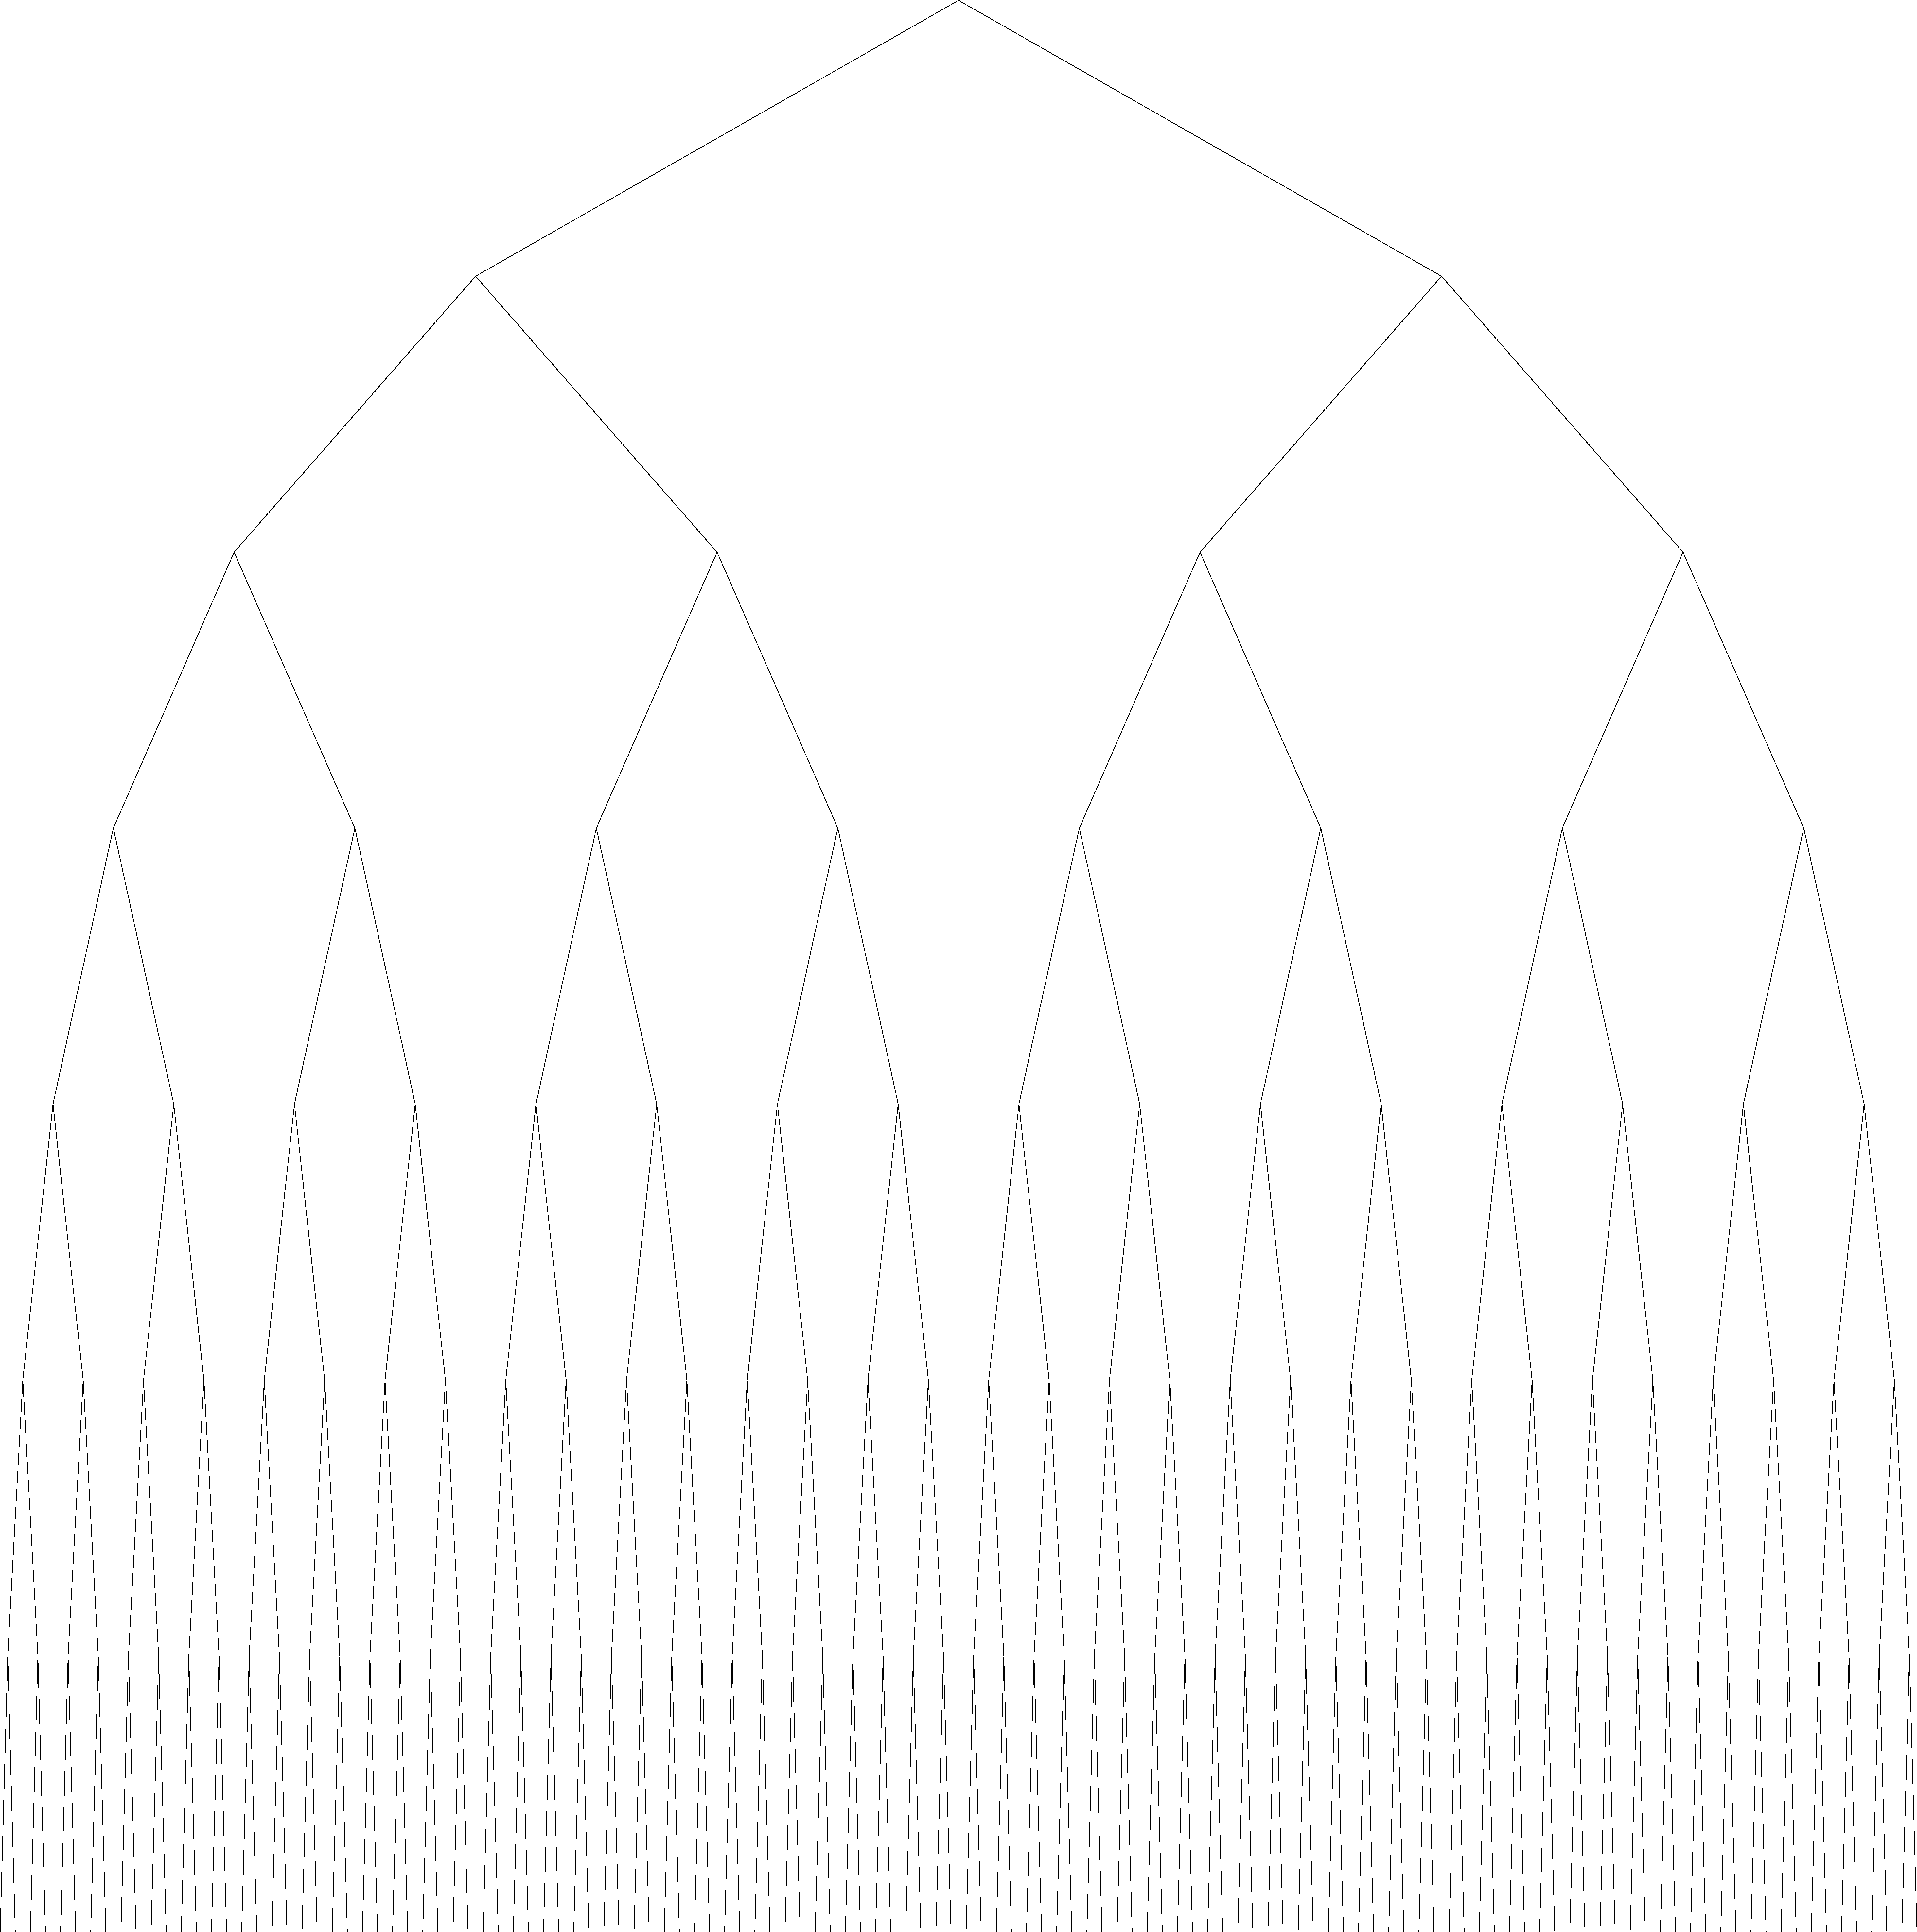
\includegraphics[width=0.8\linewidth]{reso/plain.pdf}
\end{center}

Lorsqu'on obtient une contradiction (racine de l'arbre rouge de la figure
suivante), on peut identifier précisément quelles ont été les décisions qui ont
mené à cette contradiction (branches en bleu) :
\begin{center}
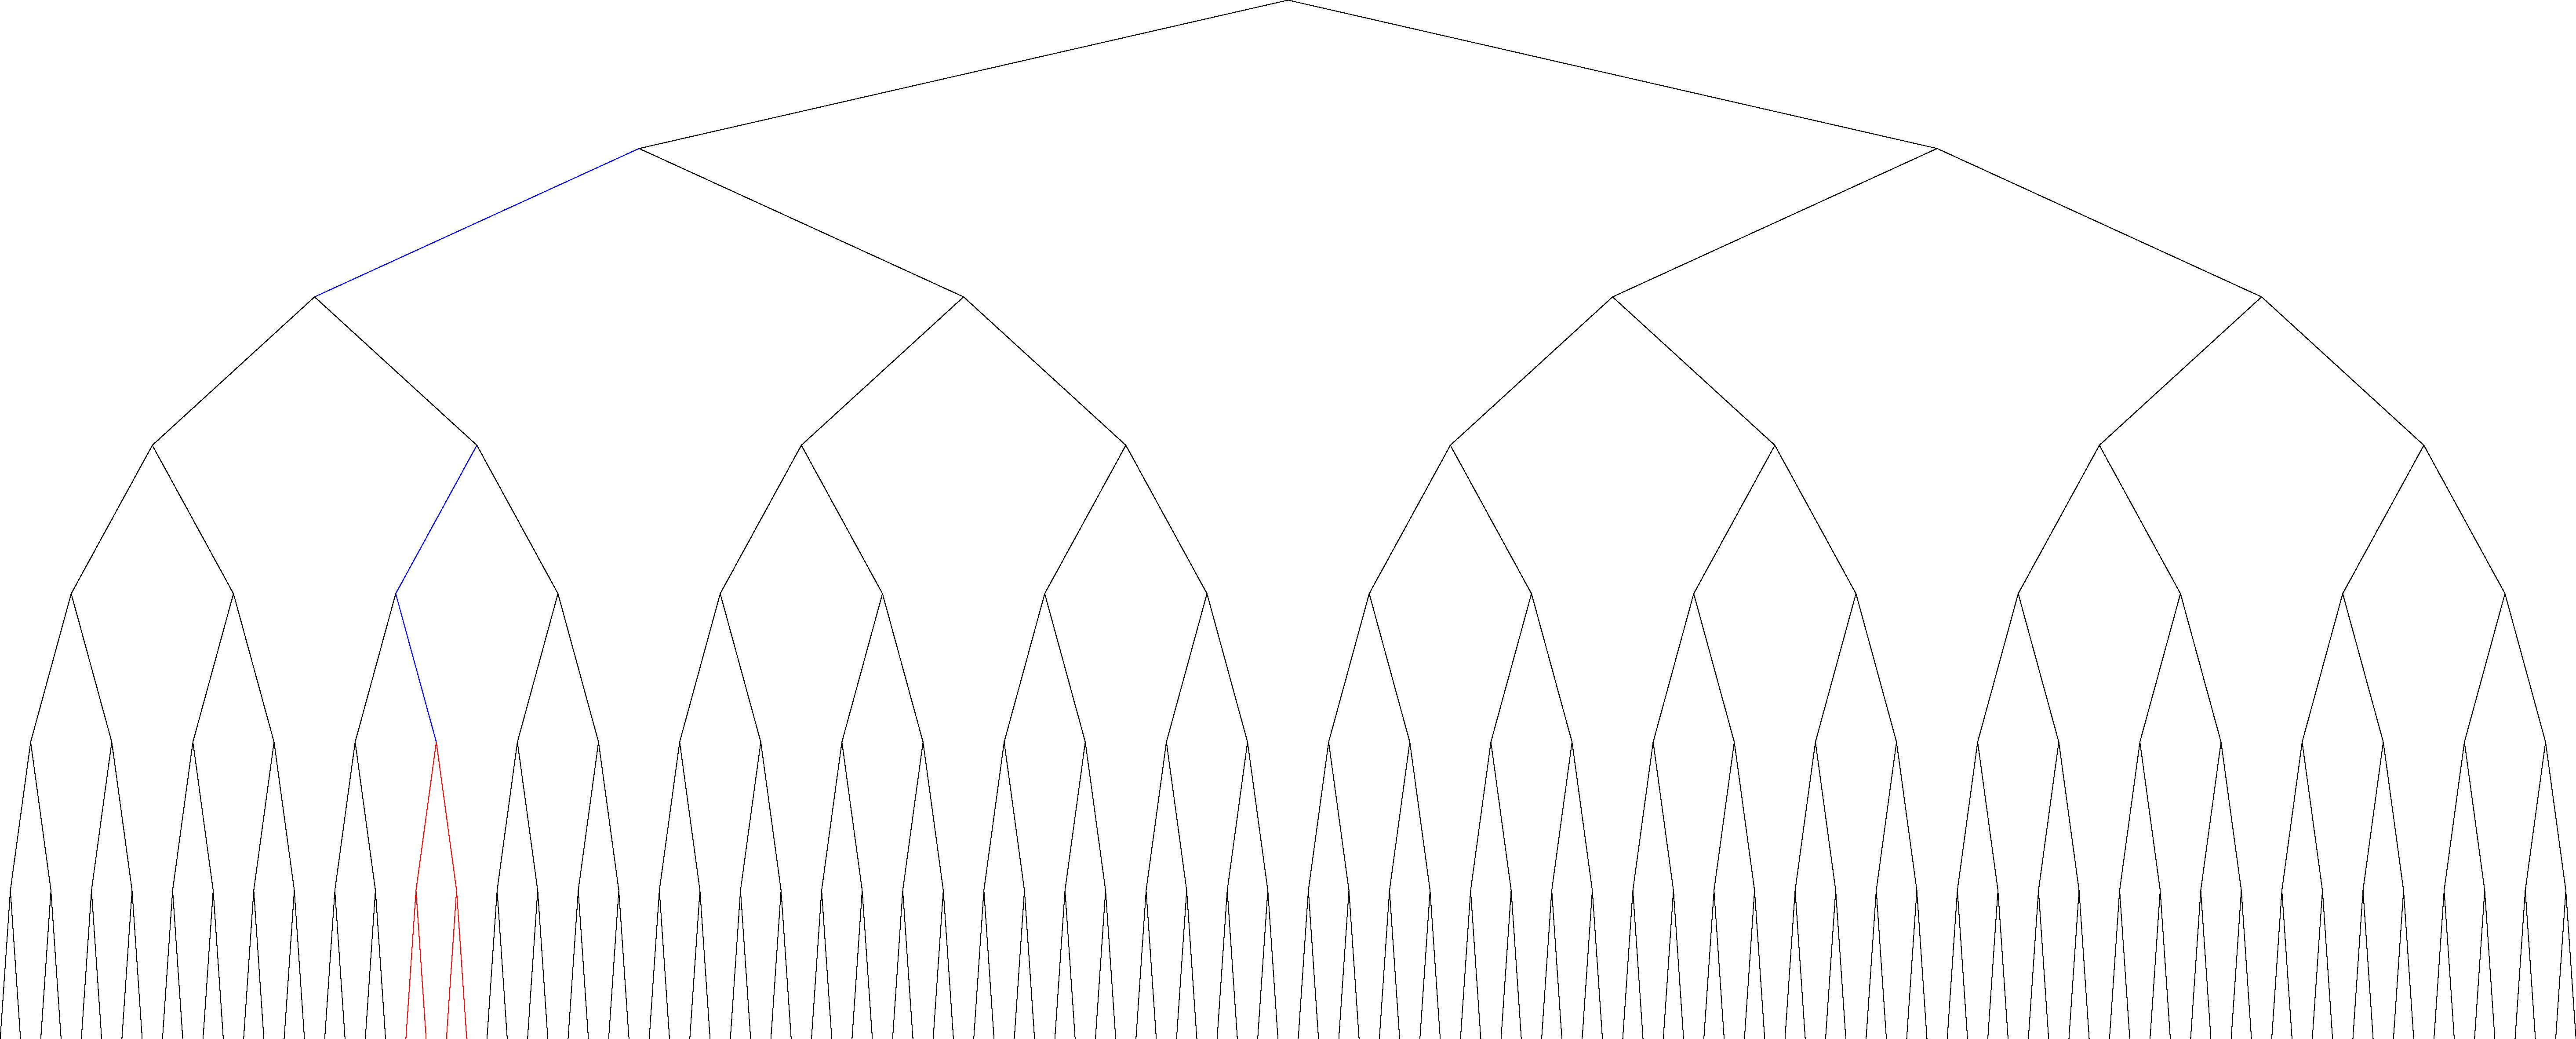
\includegraphics[width=0.8\linewidth]{reso/error.pdf}
\end{center}

On peut alors éliminer de l'espace de recherche tous les sous-arbres vérifiant
la même condition (en rouge sur l'arbre suivant) :
\begin{center}
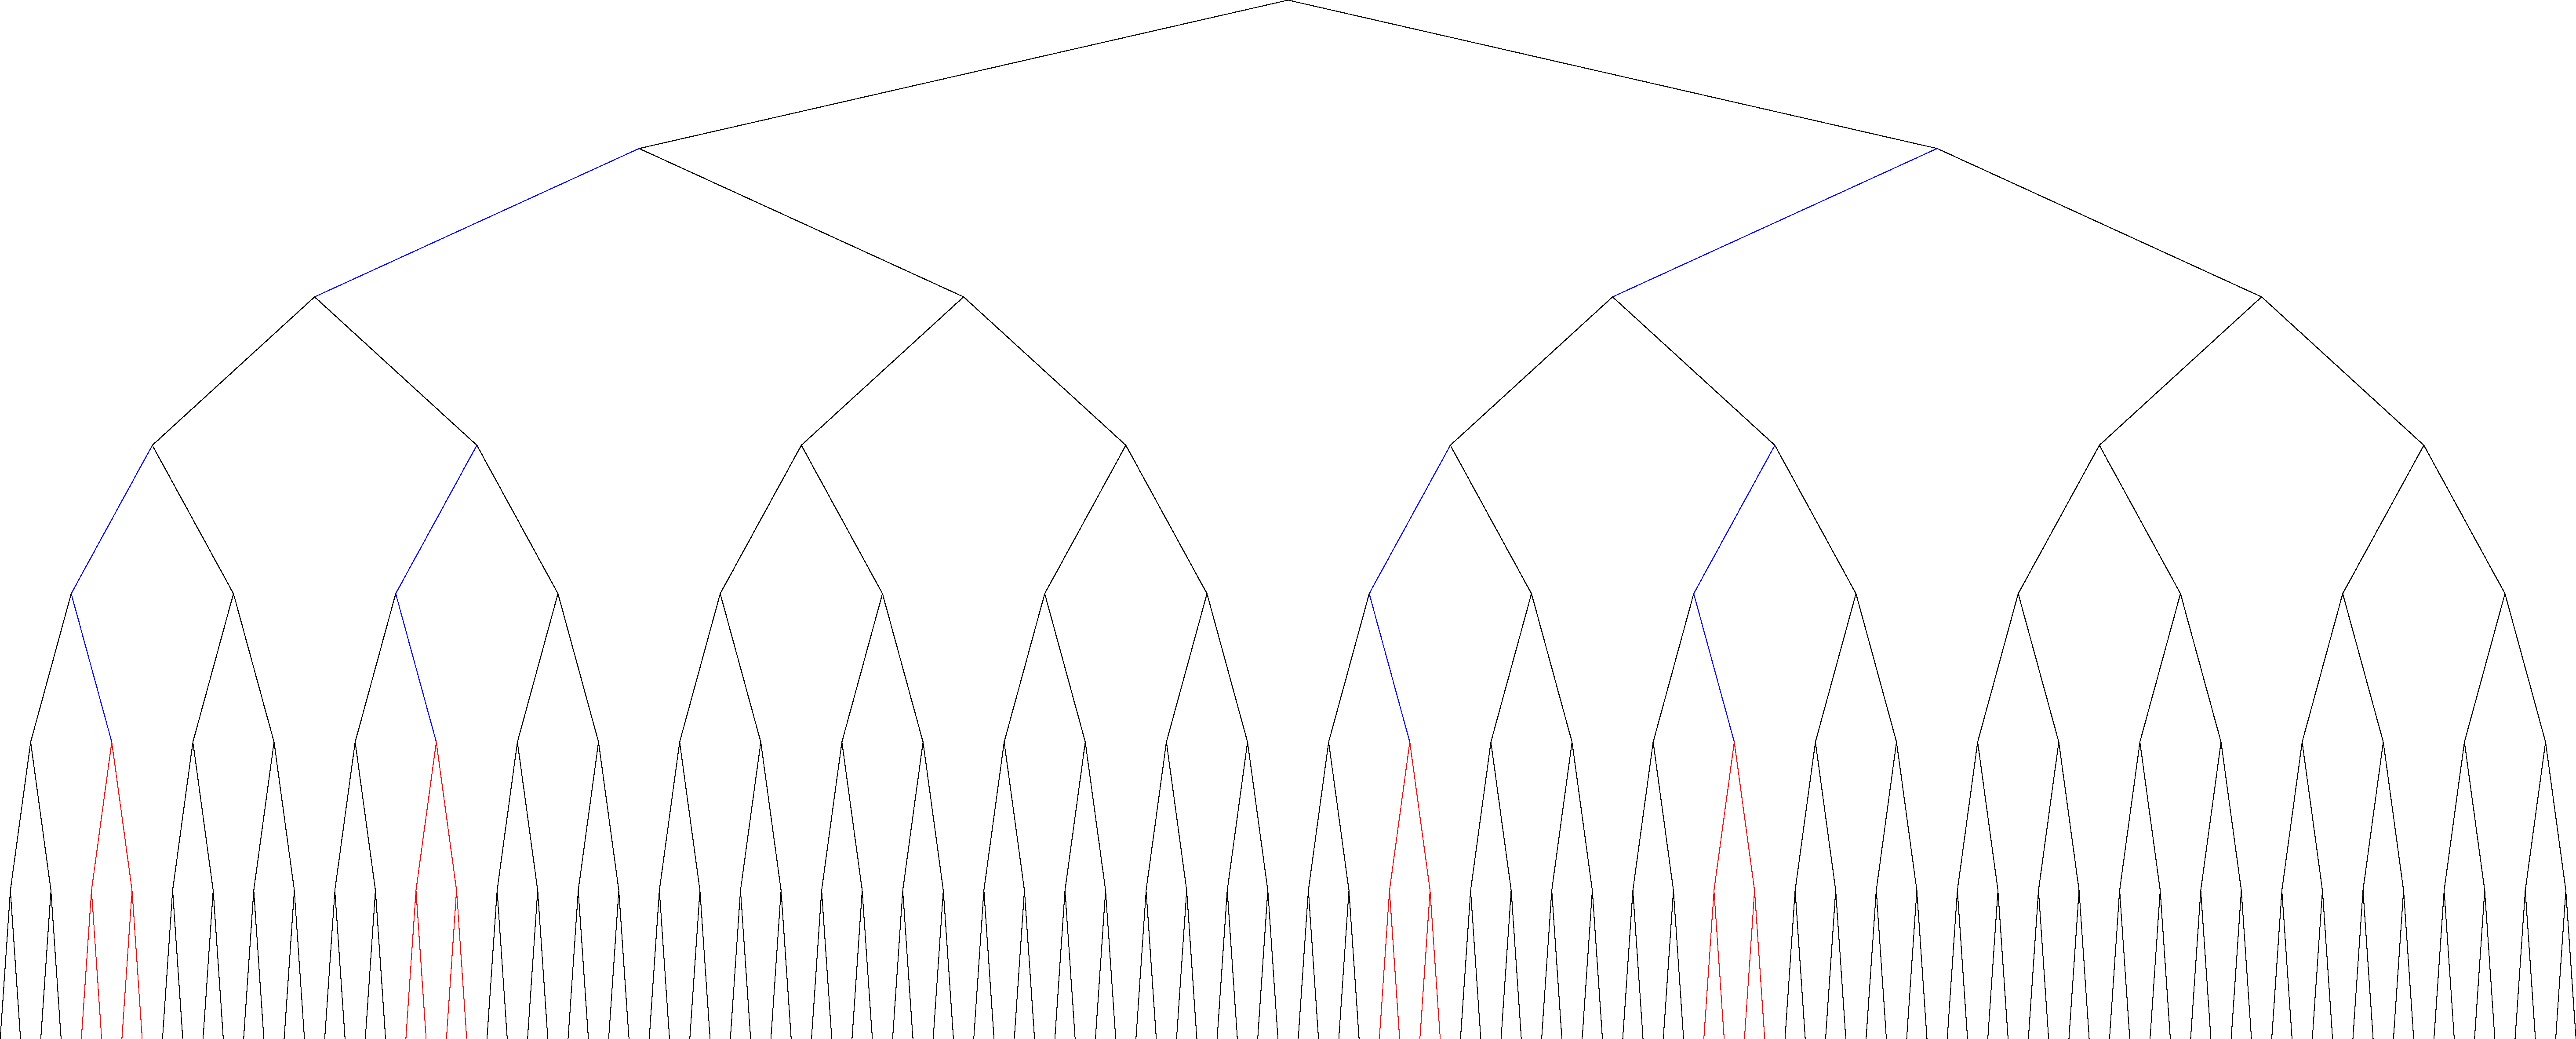
\includegraphics[width=0.8\linewidth]{reso/eliminated.pdf}
\end{center}

En pratique, on élimine ces parties en ajoutant une clause qui représente
l'erreur.

Pour déterminer cette clause, on considère la clause $c$ dont tous les litéraux
sont faux. Pour chaque litéral faux $x$ de cette clause, soit on ajoute $x$ à
la clause apprise, soit on applique le même raisonnement à la clause qui a
propagée $x$ si $x$ n'a pas été fixé. Pour remonter au premier UIP, il faut
continuer à remonter jusqu'à ce que la clause apprise ne contienne que des
variables fixées.

Afin de bien comprendre, considérons le problème SAT :
\[ (h\vee\neg b) \wedge (e\vee\neg h\vee\neg c)
   \wedge (\neg g\vee\neg d\vee\neg c) \wedge (a\vee\neg h\vee d)
   \wedge (a\vee\neg d\vee\neg e\vee g)\]

Supposons que l'on fixe $a$ à faux, $b$ à vrai et $c$ à vrai. Lorsqu'on fixe
$b$ à vrai, la clause 1 fixe $h$ à vrai, donc la clause 4 fixe $d$ à vrai.
Puis, en fixant $c$ à vrai, on obtient $e$ vrai d'après la clause 2 et $g$
faux d'après la clause 3. On a alors un conflit, puisque la clause 5 est alors
fausse. En appliquant la méthode précédente, on obtient alors le graphe
suivant (en rouge la litéraux faux, en vert ceux vrai et en bleu ce qui sont
décidés) :
\begin{center}
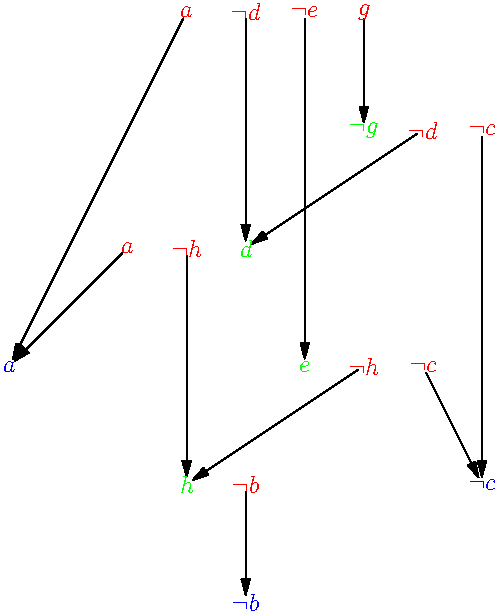
\includegraphics[width=0.5\linewidth]{reso/graph.pdf}
\end{center}

En remontant à la première UIP, la clause alors apprise est
$a\vee\neg b\vee\neg c$. On peut ici prouver que cette clause peut se déduire
du problème (et donc que son ajout ne change rien à la satisfiabilité du
problème) en utilisant la résolution :
\begin{align*}
    (a\vee\neg d\vee\neg e\vee {\color{green}g})
    \wedge({\color{green}\neg g}\vee\neg d\vee\neg c)
        &\implies a\vee\neg d\vee\neg e\vee\neg c \\
    (a\vee{\color{green}\neg d}\vee\neg e\vee\neg c)
    \wedge(a\vee\neg h\vee{\color{green} d})
        &\implies a\vee\neg e\vee\neg c\vee\neg h \\
    (e\vee{\color{green}\neg e}\vee\neg c\vee\neg h)
    \wedge({\color{green}e}\vee\neg h\vee\neg c)
        &\implies a\vee\neg c\vee\neg h \\
    (a\vee\neg c\vee{\color{green}\neg h})\wedge({\color{green} h}\vee\neg b)
        &\implies a\vee\neg b\vee\neg c\\
\end{align*}

\subsection{Heuristiques dans le choix de la variable}\label{decision}
Dans le cas de formules non satisfiables, tout l'arbre de recherche sera
exploré. Cependant, si la formule est satisfiable, on peut se demander s'il
y a des variables qui sont plus propices de mener à une solution du problème.
\idee{Trouver une heuristique adaptée pour HIPP}

Une des heuristiques les plus efficaces est \emph{VSIDS} pour \emph{Variable
State Independent Decaying Sum}. Ce terme décrit plus précisément une famille
d'heuristiques. L'idée est d'associer à chaque variable un score nommé
\emph{activité}, initialisé à $0$. Chaque fois qu'une clause est apprise,
un ensemble de variables est choisit et leur activité est augmenté d'une
certaine grandeur appelé le \emph{additive bump}, usuellement 1. Enfin, tout
les $i$ conflits ($i=1$ pour les implémentations modernes tels \emph{miniSAT}),
le score de toutes les variables est multiplié par une grandeur
$0 < \alpha < 1$ appelée \emph{multiplicative decay}. Lorsqu'une variable doit
être choisie, c'est celle avec le plus grand score qui est sélectionnée.

Une autre heuristique, par exemple implémentée dans \emph{Grasp}, est
\emph{DLIS} pour \emph{Dynamic Largest Individual Sum}. Pour chaque variable
$x$ on associe deux grandeurs : $C_{x,p}$ le nombre de clauses non résolues
dans lesquelles $x$ apparait positivement et $C_{x,n}$ le nombre de clauses non
résolues où $x$ apparait négativement. Lors du branchage, on considère $x$ la
variable telle que $C_{x,p}$ soit maximal et $y$ telle que $C_{y,n}$ soit
maximal. Si $C_{x,p} > C_{y,n}$, on assigne $x$ à vrai, sinon on assigne $y$ à
faux.

La méthode \emph{JW} pour \emph{Jeroslow-Wang} consiste à attribuer à chaque
variable un poids qui dépend des longueurs des clauses dans lesquelles elle
intervient, puis de sélectionner celles de poids maximal, afin de favoriser
les variables qui sont dans des clauses courtes. Pour $l$ une variable, en
notant $\phi$ l'ensemble des clauses non résolues, le poids attribué est :
$J(l) = \sum_{l\in\omega,\omega\in\phi} 2^{-|\omega|}$

L'heuristique \emph{MOM} pour {Maximum Occurrence of clauses of Minimum size}
se base sur la même idée de favoriser les variables intervenant dans des
clauses de petite taille, avec en plus une tendance vers les variables qui
sont présente autant négativement que positivement. Notons $f^*(x)$ le nombre
de clauses de taille minimale contenant le littéral $x$, on sélectionne le $x$
pour lequel la grandeur $((f^*(x) + f^*(\neg x)) * 2^k + f^*(x)*f^*(\neg x)$
est maximale, avec $k$ un entier.

Ces heuristiques sont décrites dans la présentation \cite{heuriSAT}.
\emph{VSIDS} semble être l'heuristique la plus efficace en pratique\cite{VSIDS}.

\subsection{Redémarrages}\label{restart}
En pratique, on constante que sur certaines instances, les algorithmes mettent
un temps très important. C'est lié à un phénomène appelé \emph{Heavy tailed
distribution}. \todo{Détailler le principe des Heavy Tailed Distributions}
Ceci fait que dans certains cas, l'algorithme peut \emph{s'embourber} dans des
sous-arbres de l'arbre de décision. Afin d'éviter ce problème, il est
intéressant de recommencer l'exploration de l'arbre de zéros après un certain
nombre de conflits (les clauses apprises sont cependant conservées).

Une stratégie optimale dans le cas général a été mise au point\cite{luby93},
mais s'avère compliquer à utiliser en pratique.

\todo{Détailler les différentes stratégies (cf hwsat09)}.

